\newpage
\section{Auswertung}
\label{sec:Auswertung}
\subsection{Verstärkung eines gestörten Sinus-Signales}
\label{sec:Auswertung1}
%Der erste Teil der verwendeten Maschine, der Funktionsgenerator, hat einen Ausgang für Spannung, 
	%die in Amplitude, Spannungsform und Frequenz angepasst werden kann, und einen Ausgang, 
	%der parallel zum ersten Ausgang die gleiche Spannungsform und Frequenz bei konstanter Amplitude liefert.
Der Effektivwert bei Sinus-förmiger Wechselspannung ist an beiden Ausgängen \SI{4.63}{\volt}, die Frequenz $f$ beträgt $\SI{1}{\kilo\hertz}$.
Mit $U_\text{eff}=\sqrt{2}\cdot U_0$ für Sinusschwingungen ergibt sich eine Amplitude $U_0\approx \SI{6.55}{\volt}$.
Die Endspannungen $U_\text{out}$ sind in Tabelle \ref{tab:spannung} aufgetragen. 
Die angegebene Phase ist die eingestellte Phase des Phasenschiebers.
%Weiter wird das Messsignal über einen Verstärker verstärkt und mithilfe eines Bandpasses gefiltert,
	%während das Referenzsignal in einen Phasenwandler geleitet wird.
	%Beide Signale werden anschließend in dem Lock-In-Detektor gemischt und


\begin{table}
	\centering
	\begin{tabular}{c S[table-format=1.2]S[table-format=1.2]S[table-format=1.2]}
	\toprule
	{Phase \text{\Delta\phi}}&\multicolumn{3}{c}{Endspannung $U_\text{out}$ / V}\\
	&{ohne Störung}&{mit Störung}&{Differenz}\\
	\midrule
		0°		&-6.00	&-6.00	&0.00\\
		45°		&-4.00	&-4.00	&0.00\\
		90°		& 0.20	& 0.50	&0.30\\
		120°	& 2.62	& 3.00	&0.38\\
		135°	& 4.25	& 4.50	&0.25\\
		180°	& 5.81	& 6.00	&0.19\\
		225°	& 3.95	& 3.50	&-0.45\\
		270°	& 0.20	&-0.50	&-0.70\\
		315°	&-4.17	&-4.50	&-0.33\\
		360°	&-5.83	&-5.50	&0.33\\
	\bottomrule
	\end{tabular}
	\caption{Ausgangsspannung des gegebenen Signals.}
	\label{tab:spannung}
\end{table}
Diese Endspannungen $U_\text{out}$ werden in Diagramm \ref{diag:spannung} gegen die eingestellte Phase $\mathup{\Delta}\phi$ aufgetragen. 
Die Beziehung \eqref{cosinus_ausgangsspannung} wird durch die Datenpunkte verifiziert, es kommt allerdings zu einem festen Phasenversatz $\alpha$ von $\alpha\approx 180°$.
Dies ist eventuell darauf zurückzuführen, dass die Ausgänge des Funktionsgenerators und die Bauteile des Verstärkers einen permanenten Phasenversatz aufweisen oder die Leitungen einen Versatz bewirken, wodurch sich der kummulierte Versatz $\alpha$ ergibt.
Dass die Amplitude der Messkurve größer ist als die Amplitude der Theoriekurve, ist darauf zurückzuführen, dass das im Experiment benützte Referenzsignal nicht normiert-rechteckförmig, sondern sinusförmig mit Amplitude verschieden von $\SI{1}{\volt}$ ist.


Abbildung \ref{fig:stoerung} zeigt das gestörte Signal, 
neben Abweichungen von der Sinus-Form entlang der Auslenkung sind bei Aufnahmen zu verschiedenen Zeiten auch Abweichungen in Frequenz-Richtung sichtbar.
Trotz dieser Abweichungen von dem reinen Sinus-förmigen Signal werden die Werte der Messung ohne Störung gut angenähert.
Die Differenz der Spannungen ist in Tabelle \ref{tab:spannung} aufgetragen, 
die Abbildungen \ref{diag:spannung} und \ref{diag:stoerung} zeigen zueinander starke Ähnlichkeit.
Weiterer Indikator der guten Rauschunterdrückung sind die Aufnahmenserien \ref{fig:faltung} und \ref{fig:faltungstoerung}.
Gezeigt werden in Abhängigkeit von der eingestellten Phase die gefalteten Signale, die den Tiefpass erreichen.
Der paarweise Vergleich von Bildern des ungestörten und des gestörten Messsignals zeigt die Ähnlichkeit der gefalteten Signale.

\begin{figure}[hp]
	\centering
	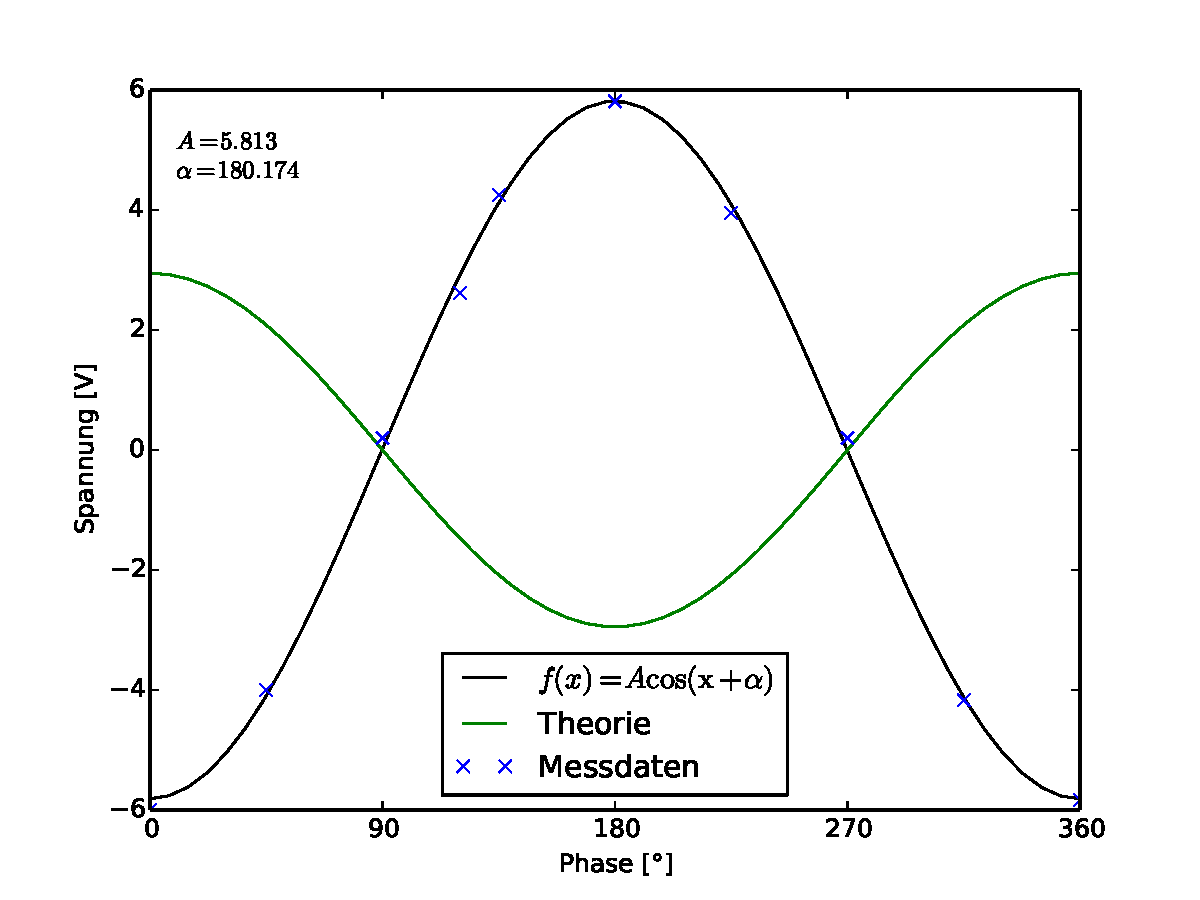
\includegraphics[width=0.8\textwidth]{Bilder/AusgangSpannung.pdf}
	\caption{Endspannung des Lock-In-Verstärkers bei Sinus-förmigen Eingang mit $U_\text{eff} = \SI{4.63}{\volt}$ und $f = \SI{300}{\hertz}$.}
	\label{diag:spannung}
\end{figure}
\begin{figure}[hp]
	\centering
	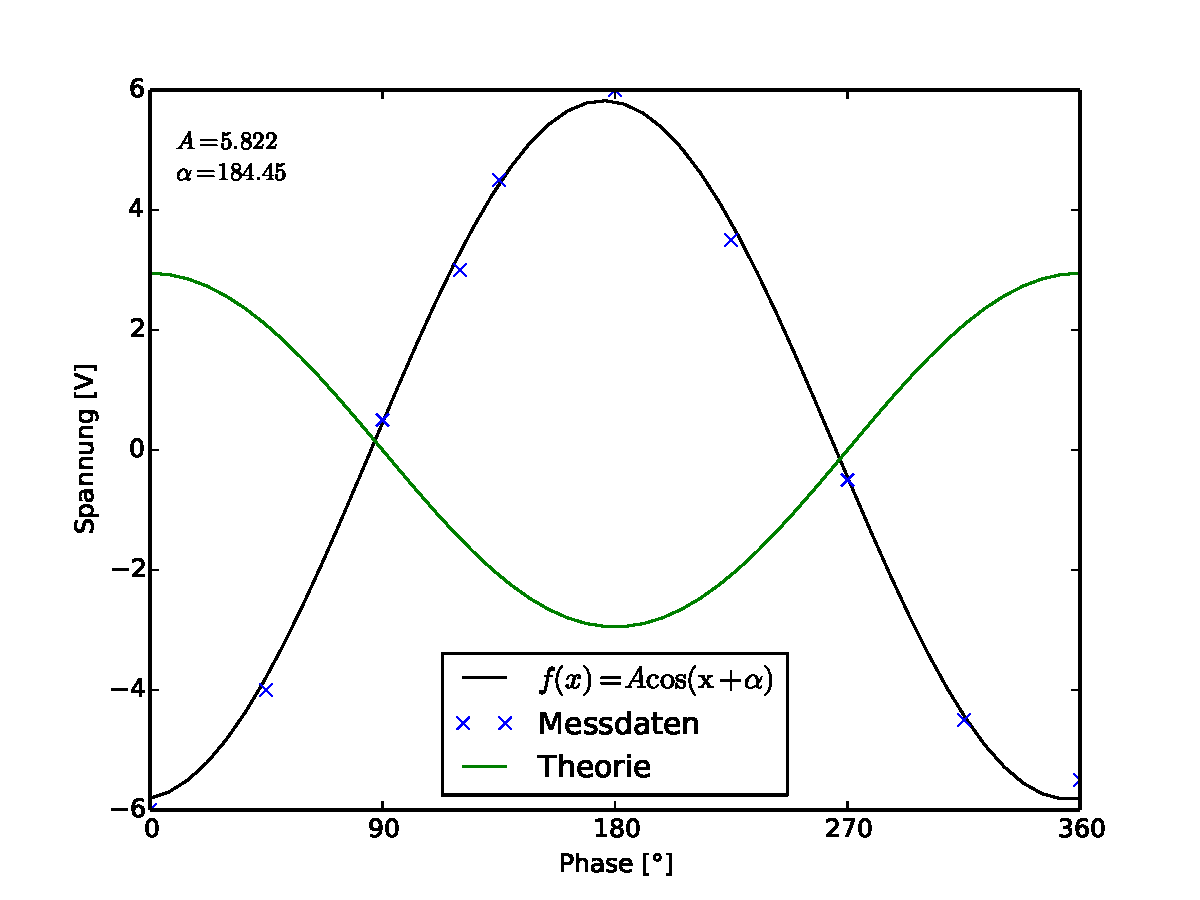
\includegraphics[width=0.8\textwidth]{Bilder/AusgangStoerung.pdf}
	\caption{Endspannung des Lock-In-Verstärkers bei gestörtem Signal.}
	\label{diag:stoerung}
\end{figure}

\begin{figure}[p]
	\centering
	\begin{subfigure}{0.32\textwidth}
		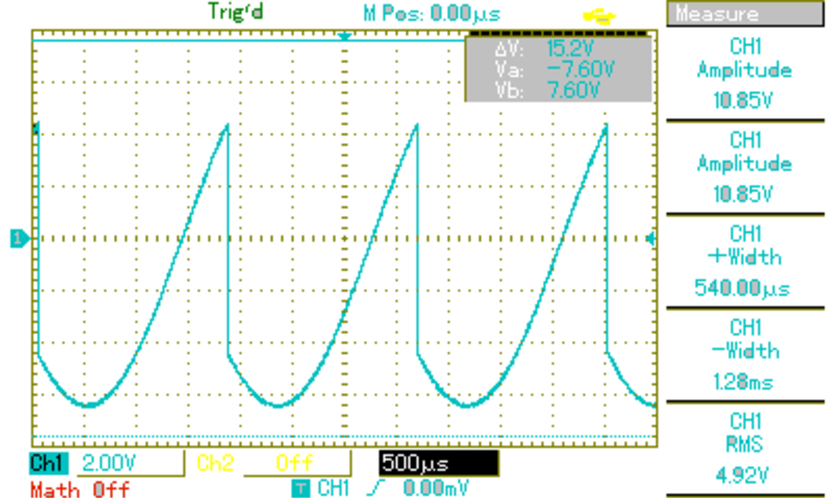
\includegraphics[width=\textwidth]{Bilder/MAP005.pdf}
		\caption{$\phi=0°$}
	\end{subfigure}
	\begin{subfigure}{0.32\textwidth}
		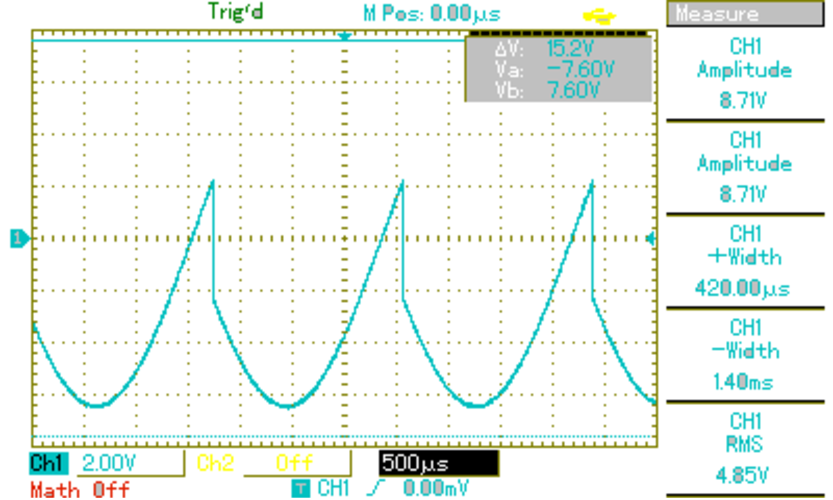
\includegraphics[width=\textwidth]{Bilder/MAP006.pdf}
		\caption{$\phi=30°$}
	\end{subfigure}
	\begin{subfigure}{0.32\textwidth}
		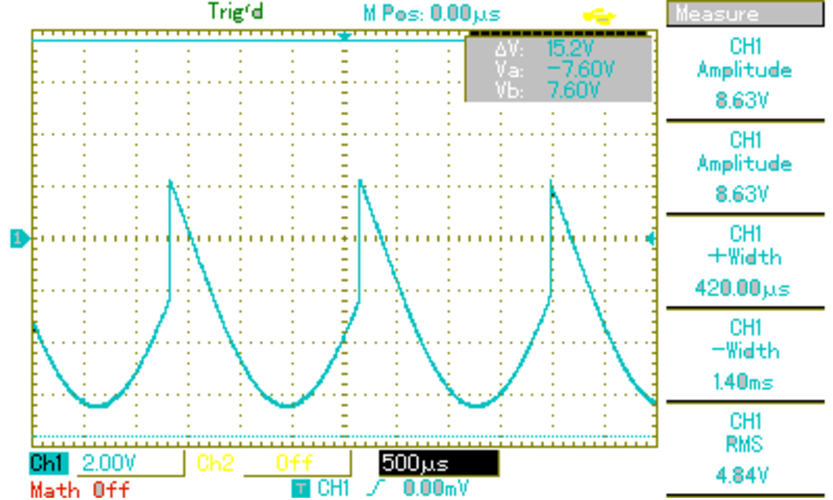
\includegraphics[width=\textwidth]{Bilder/MAP007.pdf}
		\caption{$\phi=60°$}
	\end{subfigure}
	\begin{subfigure}{0.32\textwidth}
		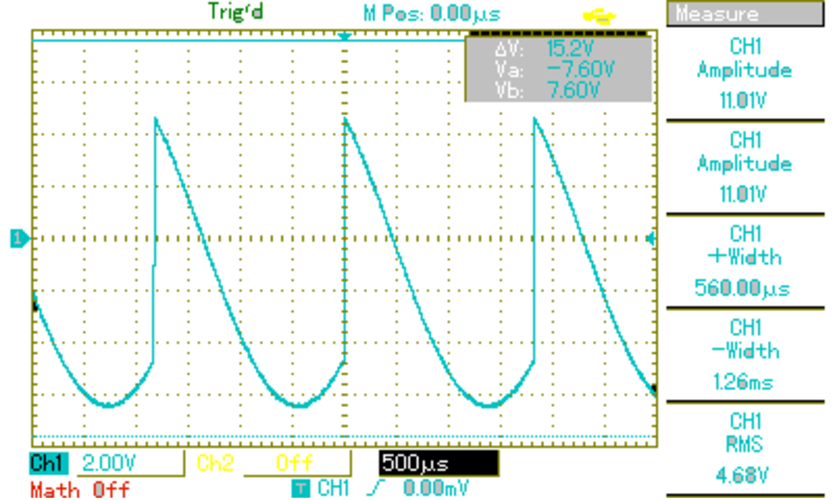
\includegraphics[width=\textwidth]{Bilder/MAP008.pdf}
		\caption{$\phi=90°$}
	\end{subfigure}
	\begin{subfigure}{0.32\textwidth}
		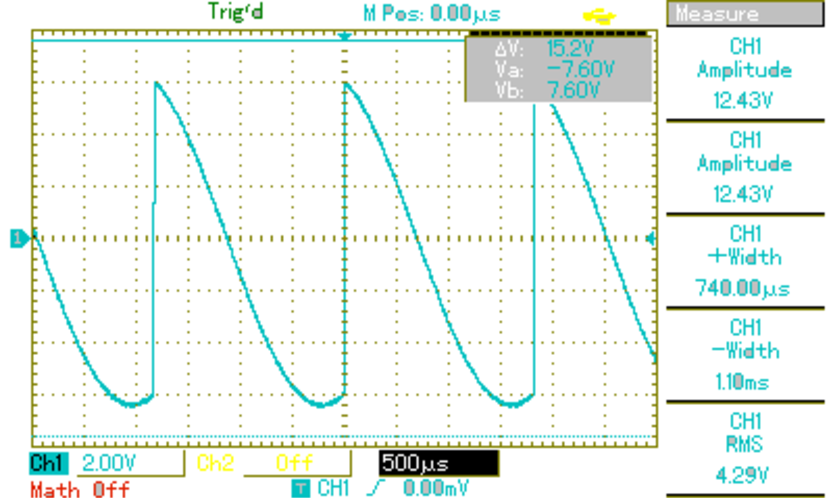
\includegraphics[width=\textwidth]{Bilder/MAP009.pdf}
		\caption{$\phi=120°$}
	\end{subfigure}
	\begin{subfigure}{0.32\textwidth}
		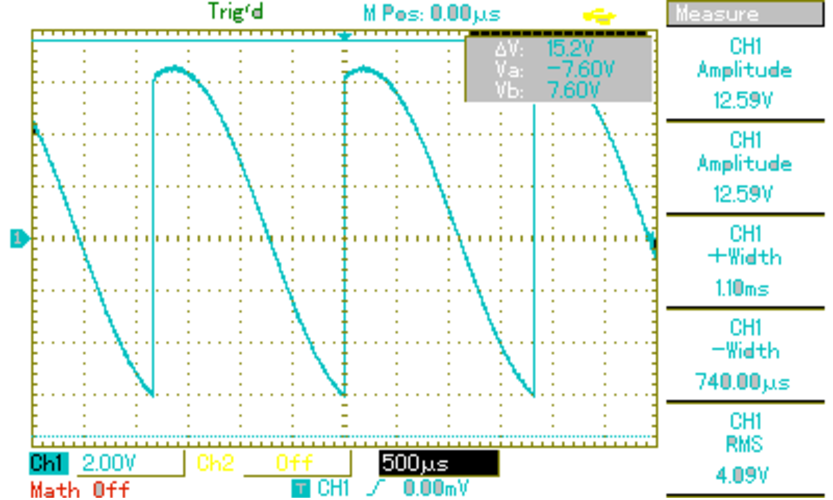
\includegraphics[width=\textwidth]{Bilder/MAP010.pdf}
		\caption{$\phi=150°$}
	\end{subfigure}
	\begin{subfigure}{0.32\textwidth}
		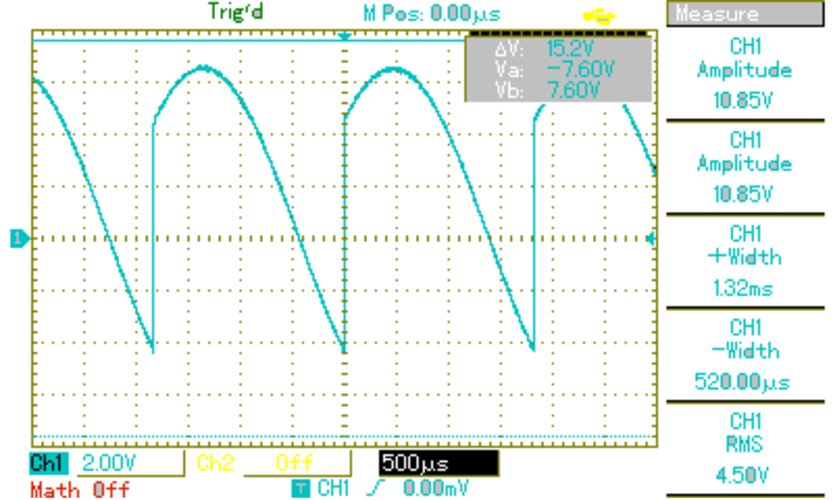
\includegraphics[width=\textwidth]{Bilder/MAP011.pdf}
		\caption{$\phi=180°$}
	\end{subfigure}
	\begin{subfigure}{0.32\textwidth}
		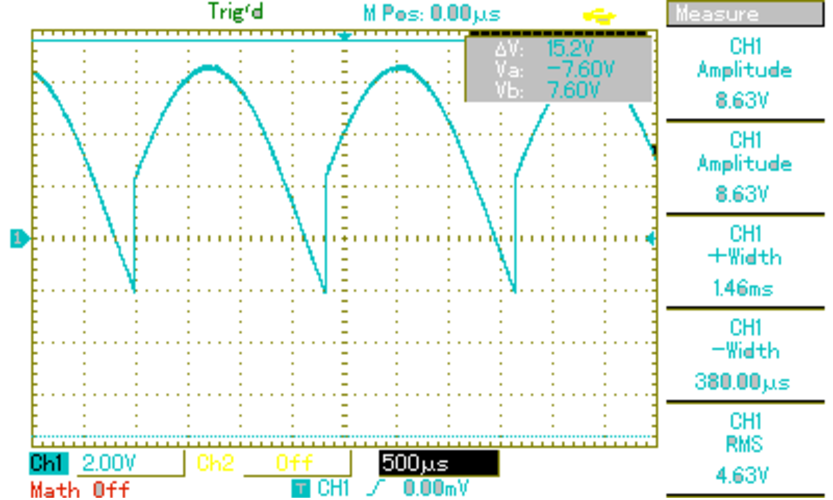
\includegraphics[width=\textwidth]{Bilder/MAP012.pdf}
		\caption{$\phi=210°$}
	\end{subfigure}
	\begin{subfigure}{0.32\textwidth}
		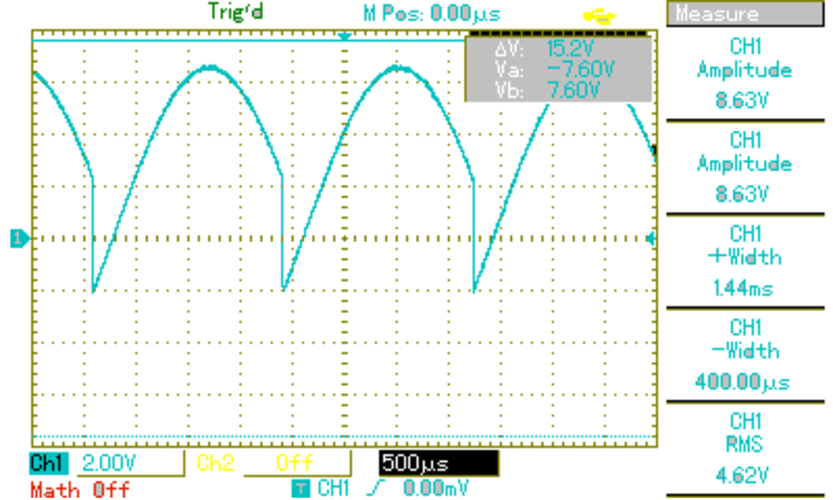
\includegraphics[width=\textwidth]{Bilder/MAP013.pdf}
		\caption{$\phi=240°$}
	\end{subfigure}
	\begin{subfigure}{0.32\textwidth}
		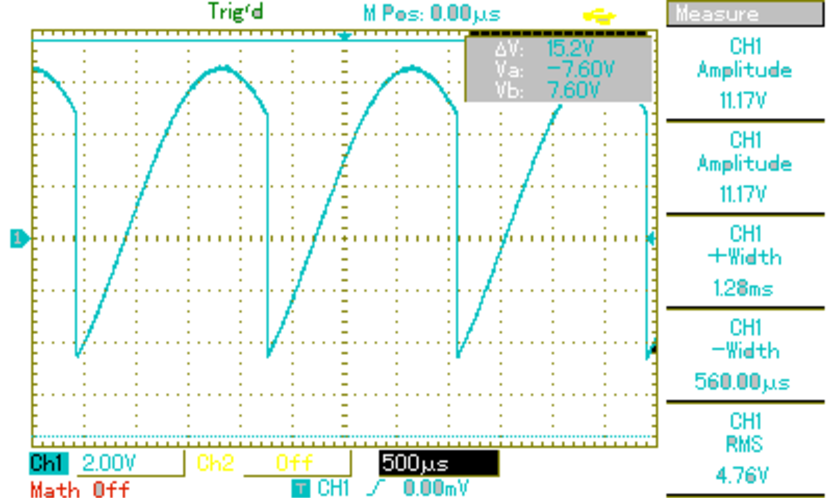
\includegraphics[width=\textwidth]{Bilder/MAP014.pdf}
		\caption{$\phi=270°$}
	\end{subfigure}
	\begin{subfigure}{0.32\textwidth}
		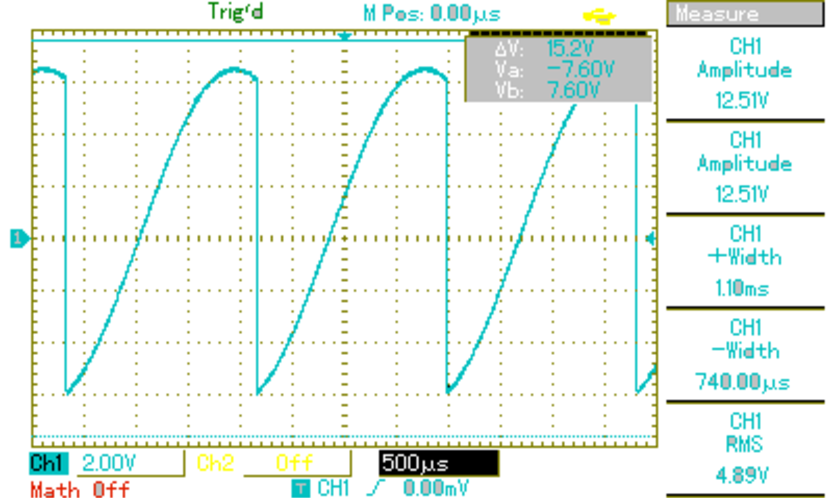
\includegraphics[width=\textwidth]{Bilder/MAP015.pdf}
		\caption{$\phi=300°$}
	\end{subfigure}
	\begin{subfigure}{0.32\textwidth}
		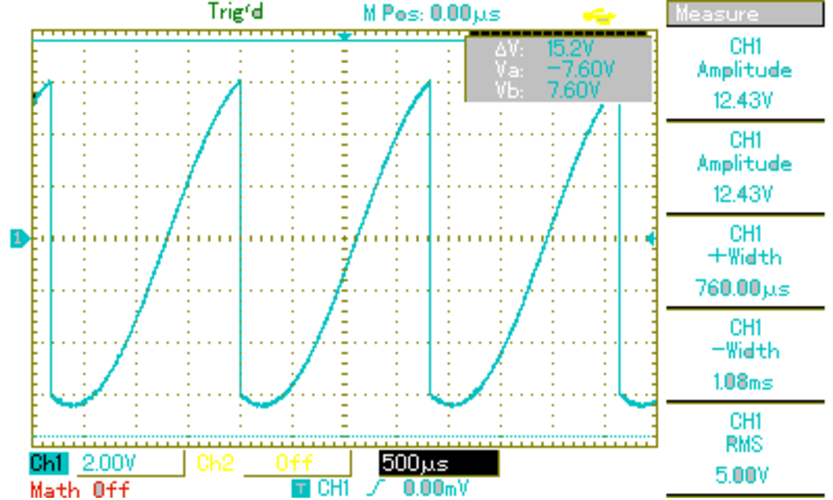
\includegraphics[width=\textwidth]{Bilder/MAP016.pdf}
		\caption{$\phi=330°$}
	\end{subfigure}
	\begin{subfigure}{0.32\textwidth}
		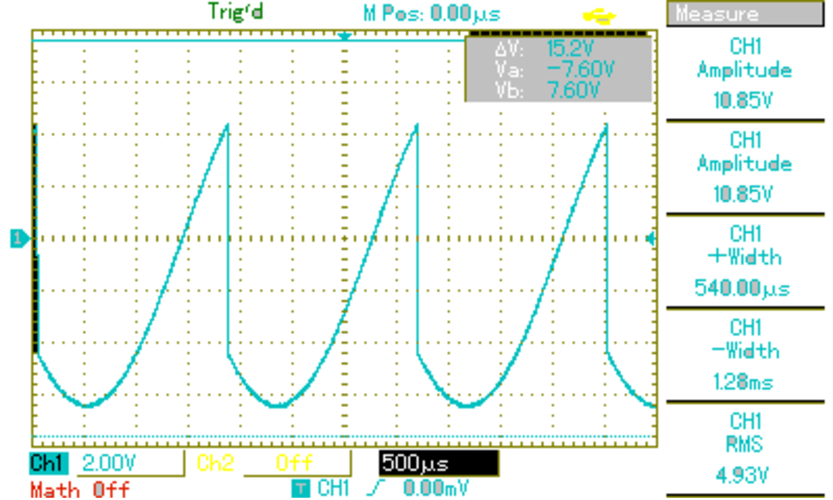
\includegraphics[width=\textwidth]{Bilder/MAP017.pdf}
		\caption{$\phi=360°$}
	\end{subfigure}
	\caption{Fotos des Oszillators: die gefalteten Signale bei variabler Phasenverschiebung. \cite{gimp}}
	\label{fig:faltung}
\end{figure}
\begin{figure}[p]
	\centering
	\begin{subfigure}{0.32\textwidth}
		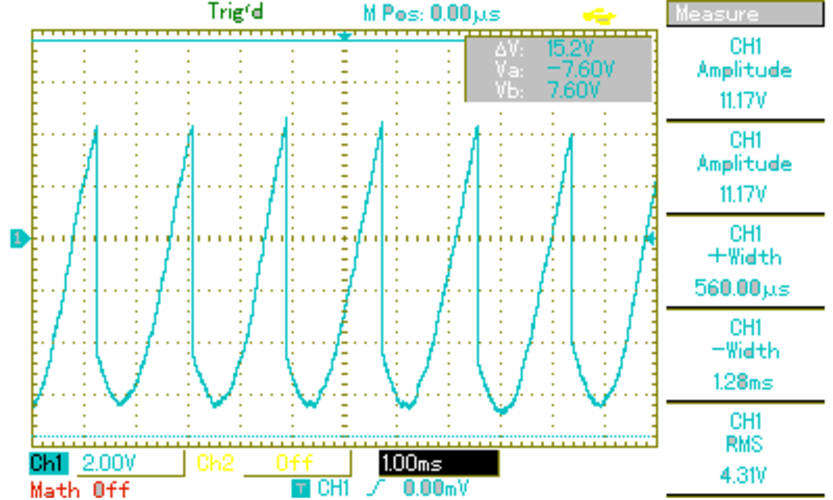
\includegraphics[width=\textwidth]{Bilder/MAP018.pdf}
		\caption{$\phi=0°$}
	\end{subfigure}
	\begin{subfigure}{0.32\textwidth}
		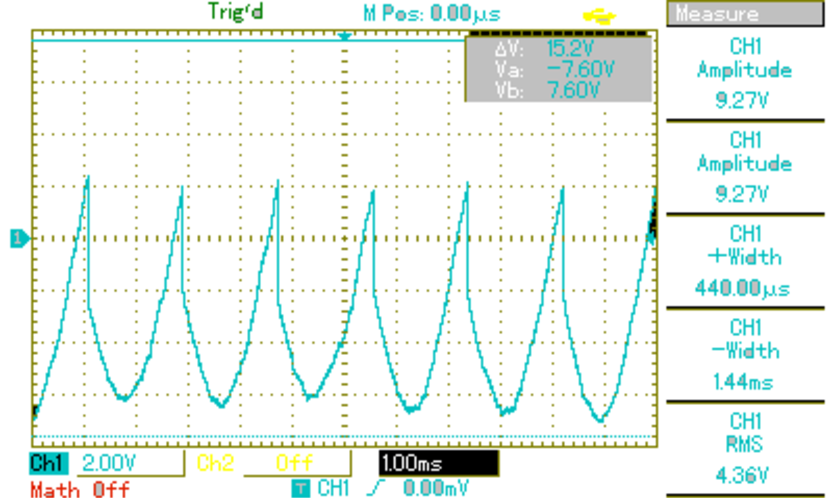
\includegraphics[width=\textwidth]{Bilder/MAP019.pdf}
		\caption{$\phi=30°$}
	\end{subfigure}
	\begin{subfigure}{0.32\textwidth}
		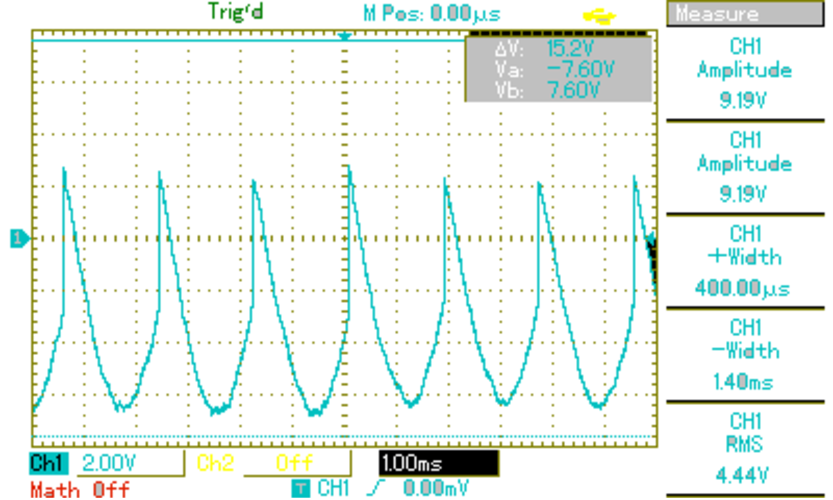
\includegraphics[width=\textwidth]{Bilder/MAP020.pdf}
		\caption{$\phi=60°$}
	\end{subfigure}
	\begin{subfigure}{0.32\textwidth}
		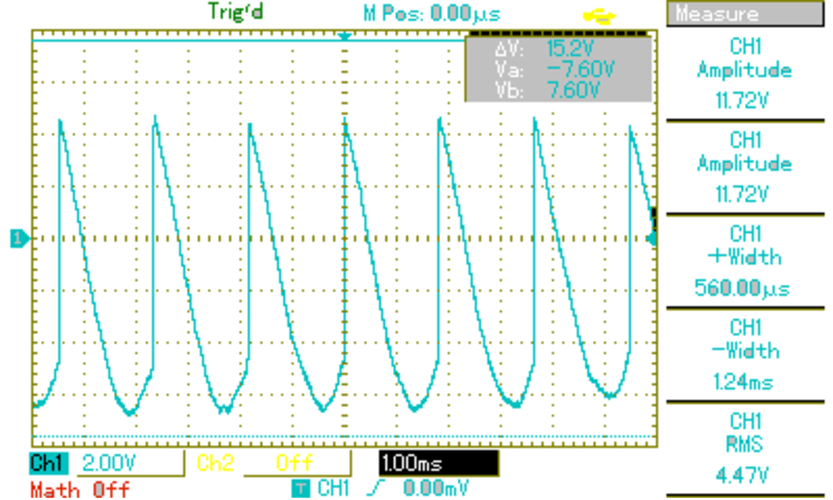
\includegraphics[width=\textwidth]{Bilder/MAP021.pdf}
		\caption{$\phi=90°$}
	\end{subfigure}
	\begin{subfigure}{0.32\textwidth}
		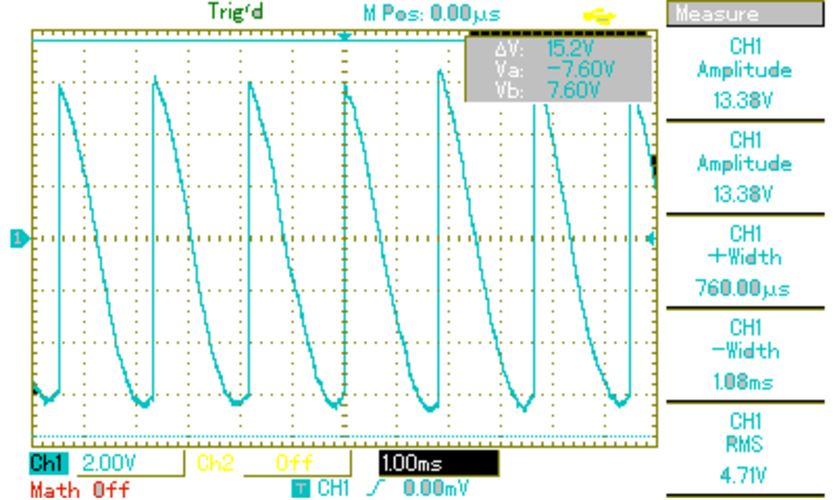
\includegraphics[width=\textwidth]{Bilder/MAP022.pdf}
		\caption{$\phi=120°$}
	\end{subfigure}
	\begin{subfigure}{0.32\textwidth}
		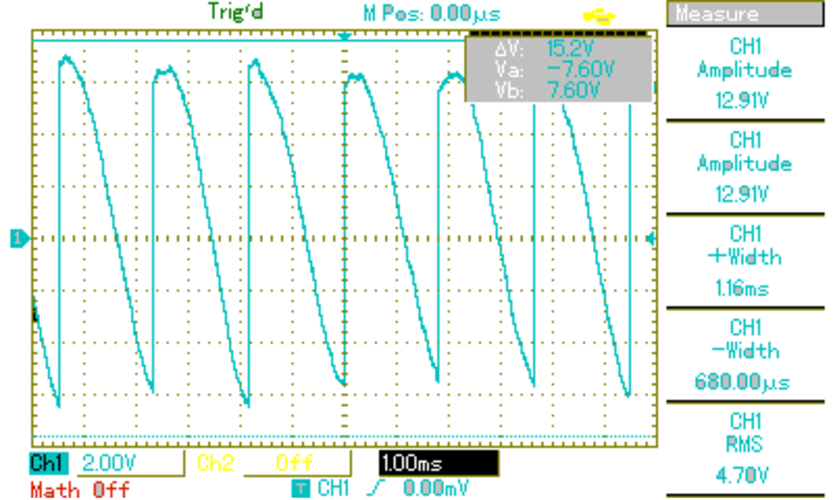
\includegraphics[width=\textwidth]{Bilder/MAP023.pdf}
		\caption{$\phi=150°$}
	\end{subfigure}
	\begin{subfigure}{0.32\textwidth}
		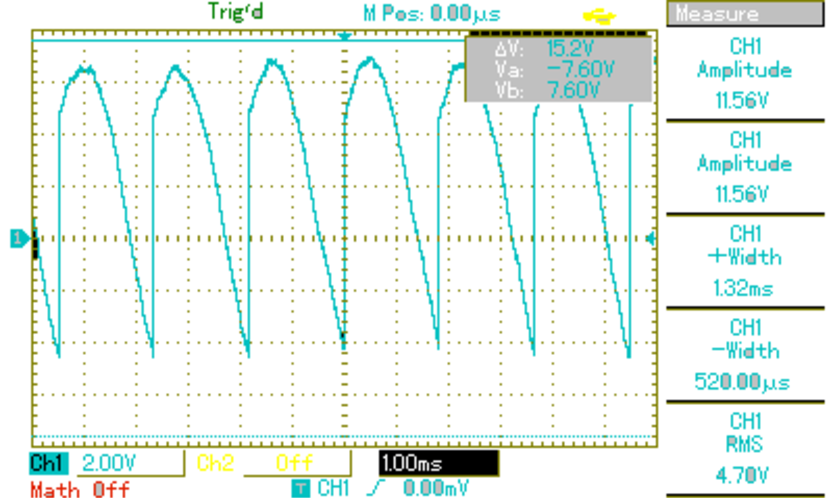
\includegraphics[width=\textwidth]{Bilder/MAP024.pdf}
		\caption{$\phi=180°$}
	\end{subfigure}
	\begin{subfigure}{0.32\textwidth}
		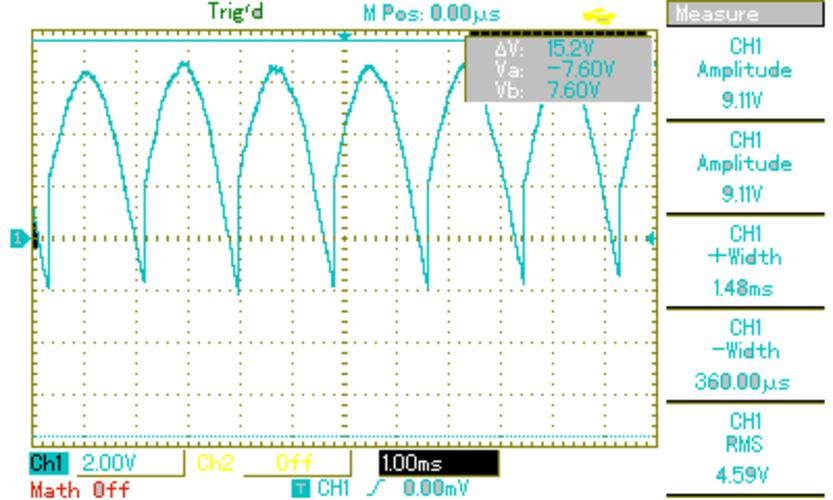
\includegraphics[width=\textwidth]{Bilder/MAP025.pdf}
		\caption{$\phi=210°$}
	\end{subfigure}
	\begin{subfigure}{0.32\textwidth}
		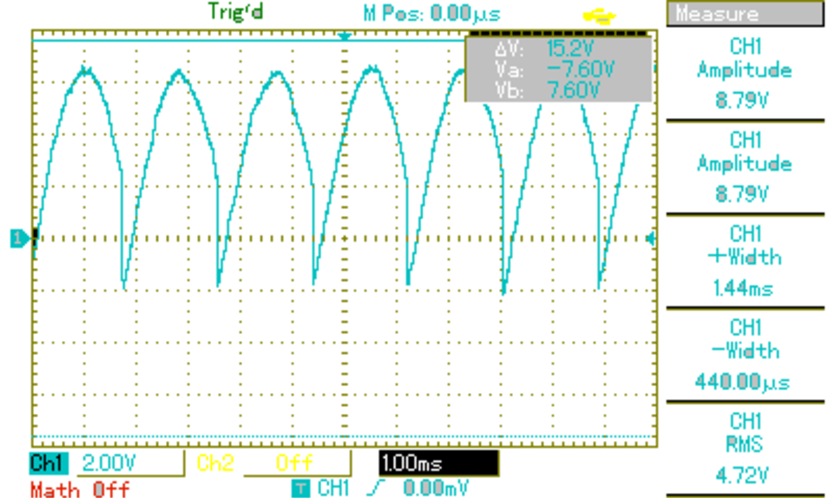
\includegraphics[width=\textwidth]{Bilder/MAP026.pdf}
		\caption{$\phi=240°$}
	\end{subfigure}
	\begin{subfigure}{0.32\textwidth}
		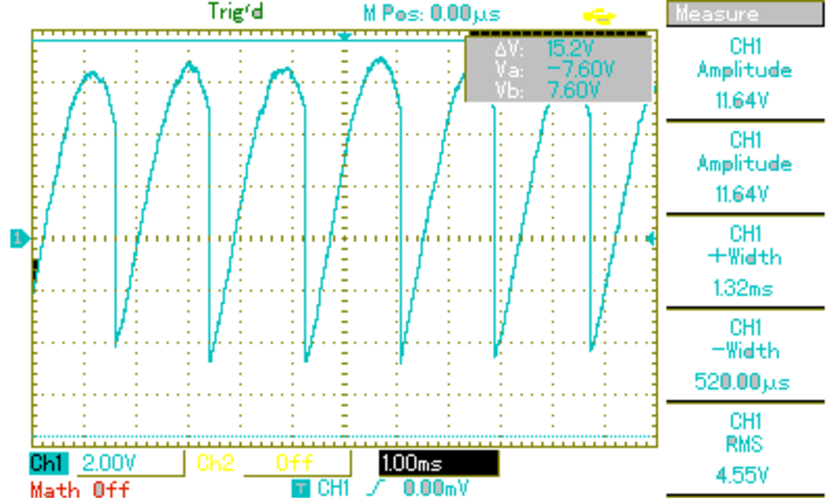
\includegraphics[width=\textwidth]{Bilder/MAP027.pdf}
		\caption{$\phi=270°$}
	\end{subfigure}
	\begin{subfigure}{0.32\textwidth}
		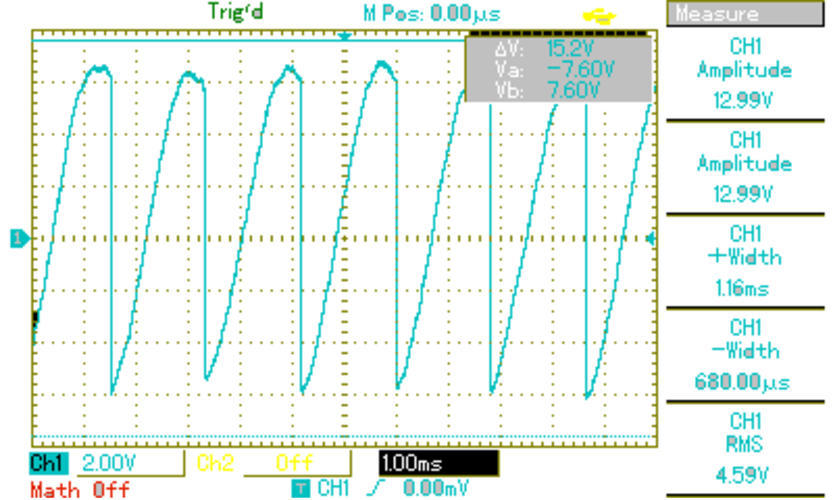
\includegraphics[width=\textwidth]{Bilder/MAP028.pdf}
		\caption{$\phi=300°$}
	\end{subfigure}
	\begin{subfigure}{0.32\textwidth}
		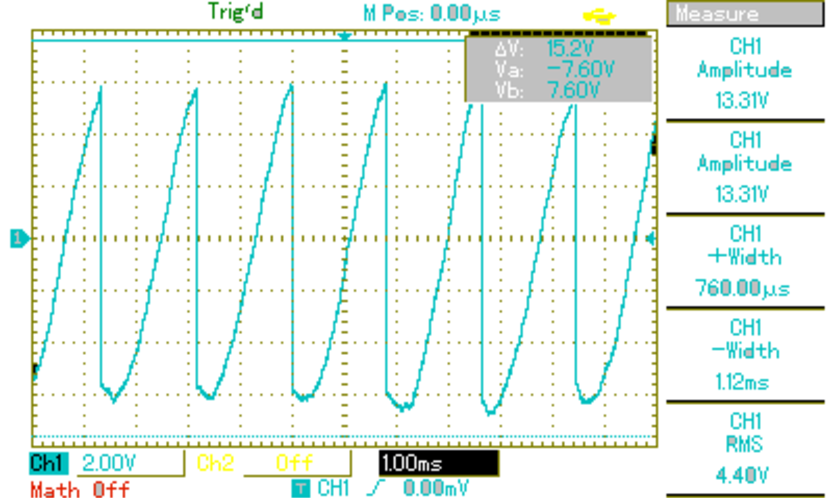
\includegraphics[width=\textwidth]{Bilder/MAP029.pdf}
		\caption{$\phi=330°$}
	\end{subfigure}
	\begin{subfigure}{0.32\textwidth}
		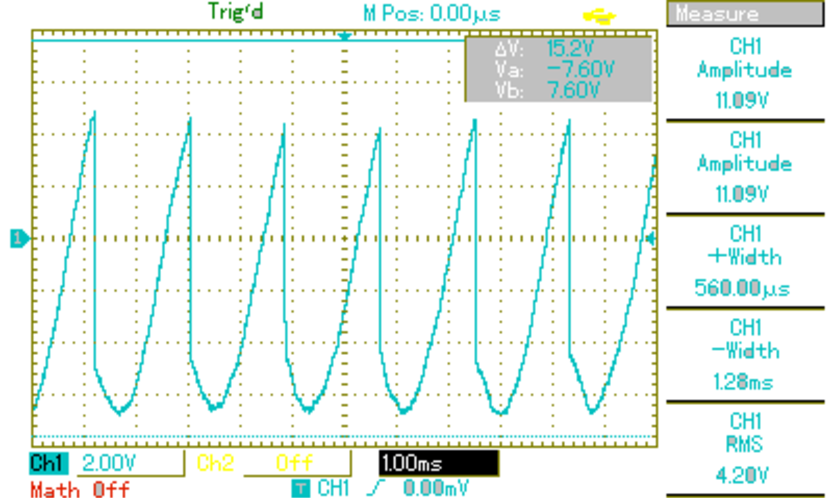
\includegraphics[width=\textwidth]{Bilder/MAP030.pdf}
		\caption{$\phi=360°$}
	\end{subfigure}
	\caption{Analog zu Abbildung \ref{fig:faltung}: Faltung des gestörten Signals. \cite{gimp}}
	\label{fig:faltungstoerung}
\end{figure}

\begin{figure}[h!]
	\centering
	\begin{subfigure}{0.49\textwidth}
		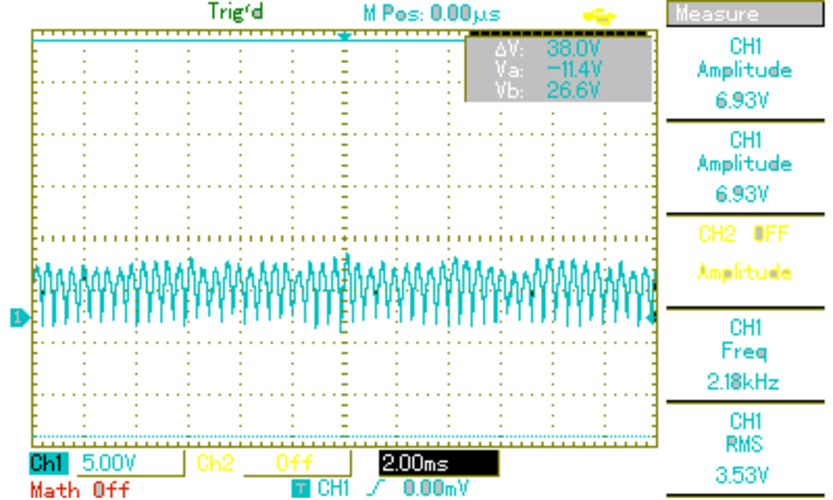
\includegraphics[width=\textwidth]{Bilder/MAP002.pdf}
	\end{subfigure}
	\begin{subfigure}{0.49\textwidth}
		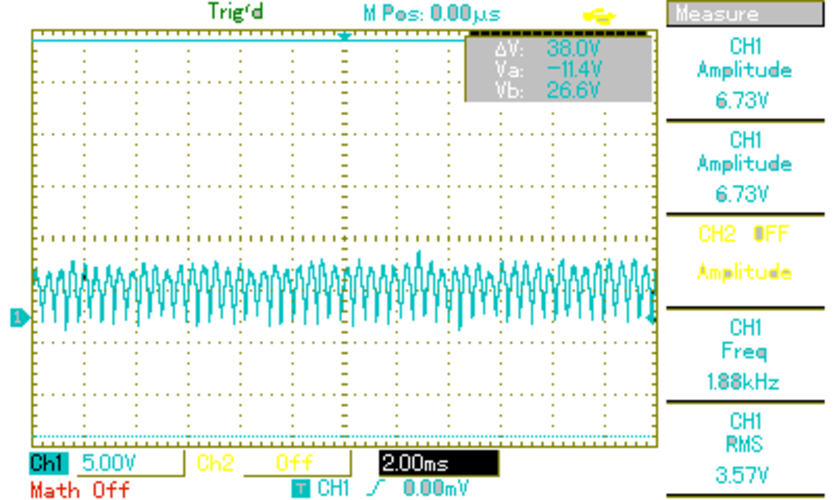
\includegraphics[width=\textwidth]{Bilder/MAP003.pdf}
	\end{subfigure}
	\caption{Fotos des Oszillators: das gestörte Messsignal zu zwei verschiedenen Zeiten. \cite{gimp}}
	\label{fig:stoerung}
\end{figure}

\subsection{Verstärkung des LED-Signales}
In Tabelle \ref{tab:led} sind die gemessenen Endspannungen $U_\text{out}$, den Abstand $a$ zwischen Photodiode und LED sowie die Gesamtverstärkung, das Produkt aus den einzelnen Verstärkungen der Bauteile, aufgetragen.
\begin{table}[h!]
	\centering
	\begin{tabular}{c S[table-format=1.2] c c S[table-format=1.4] }
	\toprule
	{Abstand a}&{Gemessene}&{Umgerechnete}&{Relative}\\
	&{Endspannung $U_\text{out}$}&{Endspannung $U_\text{out}$}&{Verstärkung}\\
	{$[\si{\meter}]$}&{$[\si{\volt}]$}&{$[\si{\volt}]$}&\\
	\midrule
		0.02&	-5 	&-5 			 & 1	\\
		0.05&	-1 	&-1 			 & 1	\\
		0.08&	-0.5 &-0.5 		 & 1	\\
		0.11&	-2 		&-0.2 	 & 10	\\
		0.14&	-1 		&-0.1 	 & 10	\\
		0.17&	-0.9 	&-0.09 	 & 10	\\
		0.20&	-6.0	 &-0.06	& 100	\\
		0.23&	-4.5 	 &-0.045 	& 100	\\
		0.26&	-3.5 	 &-0.035 	& 100	\\
		0.29&	-2.5 	 &-0.025 	& 100	\\
		0.39&	-1.0 	 &-0.01 	& 100	\\
		0.49&	-0.7 	 &-0.007 	& 100	\\
		0.59&	-0.5 	 &-0.005 	& 100	\\
		0.69&	-0.3 	 &-0.003 	& 100	\\
		0.79&	-0.25 	 &-0.0025 & 100	\\
		0.99&	-0.12 	 &-0.0012 & 100	\\
		1.19&	-0.1 	 &-0.001 	& 100	\\
	\bottomrule
	\end{tabular}
	\caption{Ausgangsspannung bei der Messung des LED-Lichtes.}
	\label{tab:led}
\end{table}
In \ref{sec:Auswertung1} ist experimentell nachgewiesen, dass der Betrag der Endspannung $U_\text{out}$ maximal wird, wenn der Phasenschieber auf Vielfache von 180° eingestellt ist.
Bei der Einstellung $\mathup{\Delta}\phi=0°$ wird eine maximale, negative Endspannung $U_\text{out}$ erwartet und so den eventuellen Einfluss des Phasenschiebers umgangen.
Das Signal, das von der Photodiode aufgenommen wird, wandelt der Lock-In-Verstärker dementsprechend in eine reine negative Gleichspannung als Endspannung.
Im Interesse der Lesbarkeit werden die negativen Spannung unter Berücksichtigung der Gesamt-Verstärkung in Diagramm \ref{diag:LED} aufgetragen.
Hierzu wird die Anfangsverstärkung als 1 definiert und die gemessenen Endspannungen durch die jeweilige relative Gesamtverstärkung dividiert.
Der näherungsweise lineare Abfall der Spannung bei doppel-logarithmischer Skalierung zeigt, dass die gemessene Intensität mit $r^{-\alpha}$ mit $\alpha \in \mathbb{R}$ abfällt.

Zur Kontrolle, dass die angegebenen Spannungen auf das LED-Signal zurückzuführen sind und nicht von Fremdeinflüssen stammen, wird die LED zeitweise abgedeckt.
Dabei geht bei einem messbaren Signal die Ausgangsspannung auf Null zurück und nimmt ihren ursprünglichen Wert an, wenn der Lichtweg zwischen LED und Photodiode frei gemacht wird.
Bei einem Abstand größer als $\SI{1.20}{\meter}$ ist trotz Verstärkung keine Ausgangsspannung zuverlässig messbar, 
die Ausgangsspannung zeigt beim Abdecken der LED keine wesentliche Änderung.

In Abbildung \ref{diag:LED} wird die Linearisierung der Messwerte vorgenommen.
Es wird eine Regression für die Funktionsklasse 
\begin{equation}
	y(x)=A\cdot x^b
\end{equation}
angesetzt, die nach der doppelten Linearisierung die Gestalt
\begin{equation}
	\underbrace{\text{ln}(y(x))}_{y_\text{lin}}=\underbrace{\text{ln}(A)}_{d_\text{lin}}+\underbrace{b}_{c_\text{lin}}\cdot \underbrace{\text{ln}(\text{exp}(x))}_{x}
\end{equation}
hat.
Für diese linearisierte Ausgleichsgerade gilt (vgl. \cite{scipy})
\begin{subequations}
	\begin{equation}
		\Delta = N \sum{x^2} - {\Bigl(\sum{x}\Bigr)}^2
	\end{equation}
	\begin{equation}
		c_{\text{lin}} = \frac{N\sum{x\cdot y} - \sum{x} \cdot \sum{y}}{\Delta}
	\end{equation}
    \begin{equation}
		d_{\text{lin}} = \frac{\sum{x^2} \cdot \sum{y} - \sum{x} \cdot \sum{x \cdot y}}{\Delta}
	\end{equation}
	% \begin{equation}
	% 	\sigma_{y} = \sqrt{\frac{\sum{(y - m_{\text{Reg}} \cdot x - b_{\text{Reg}})^2}}{N - 2}}
	% \end{equation}
	% \begin{equation}
	% 	\sigma_{m} = \sigma_{y} \sqrt{\frac{N}{\Delta}}
	% \end{equation}
	% \begin{equation}
	% 	\sigma_{b} = \sigma_{y} \sqrt{\frac{\sum{x^2}}{\Delta}}
	% \end{equation}
\end{subequations}
mit der Anzahl aller Werte N.
\begin{figure}[hbp]
	\centering
	% \begin{subfigure}{0.8\textwidth}
	% 	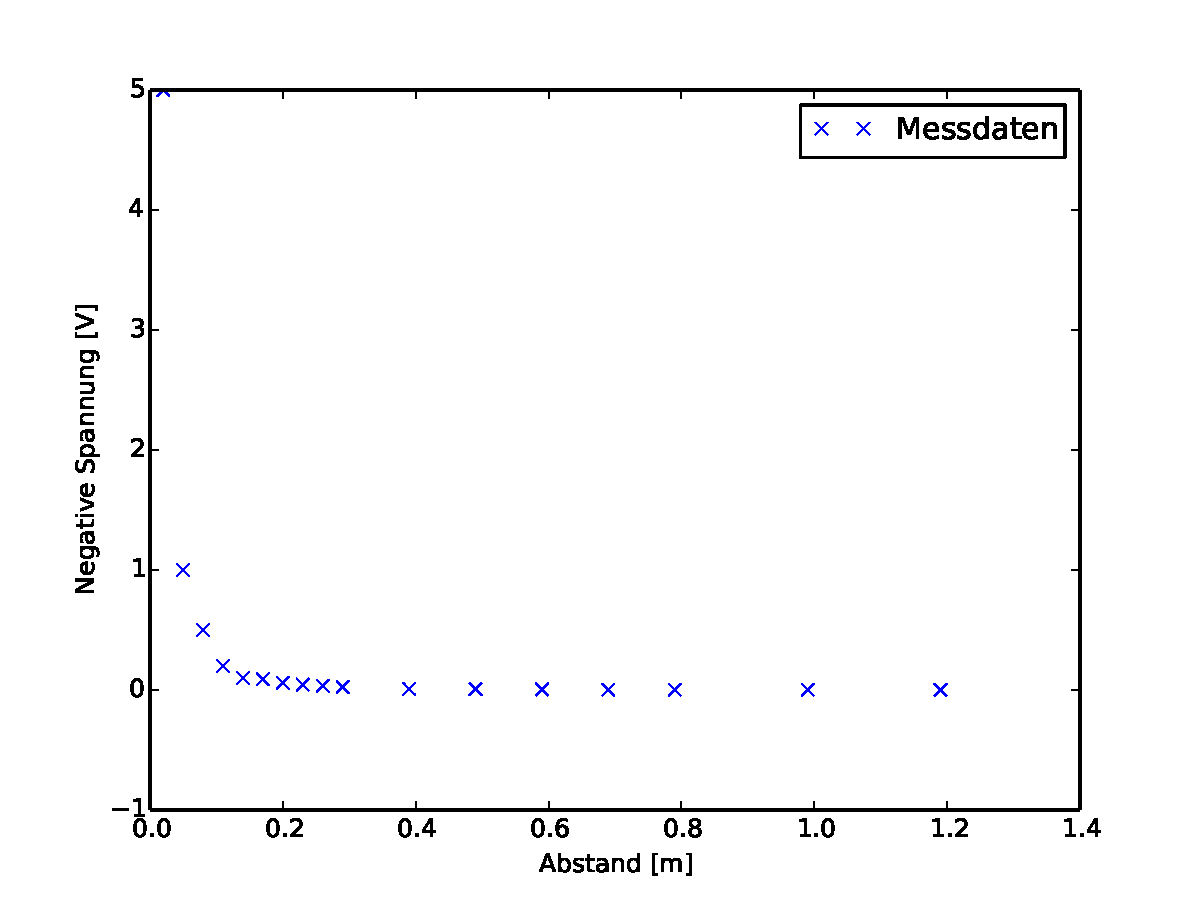
\includegraphics[width=\textwidth]{Bilder/LED.pdf}
	% 	\caption{Lineare Skalierung.}
	% \end{subfigure}
	% \begin{subfigure}{0.8\textwidth}
		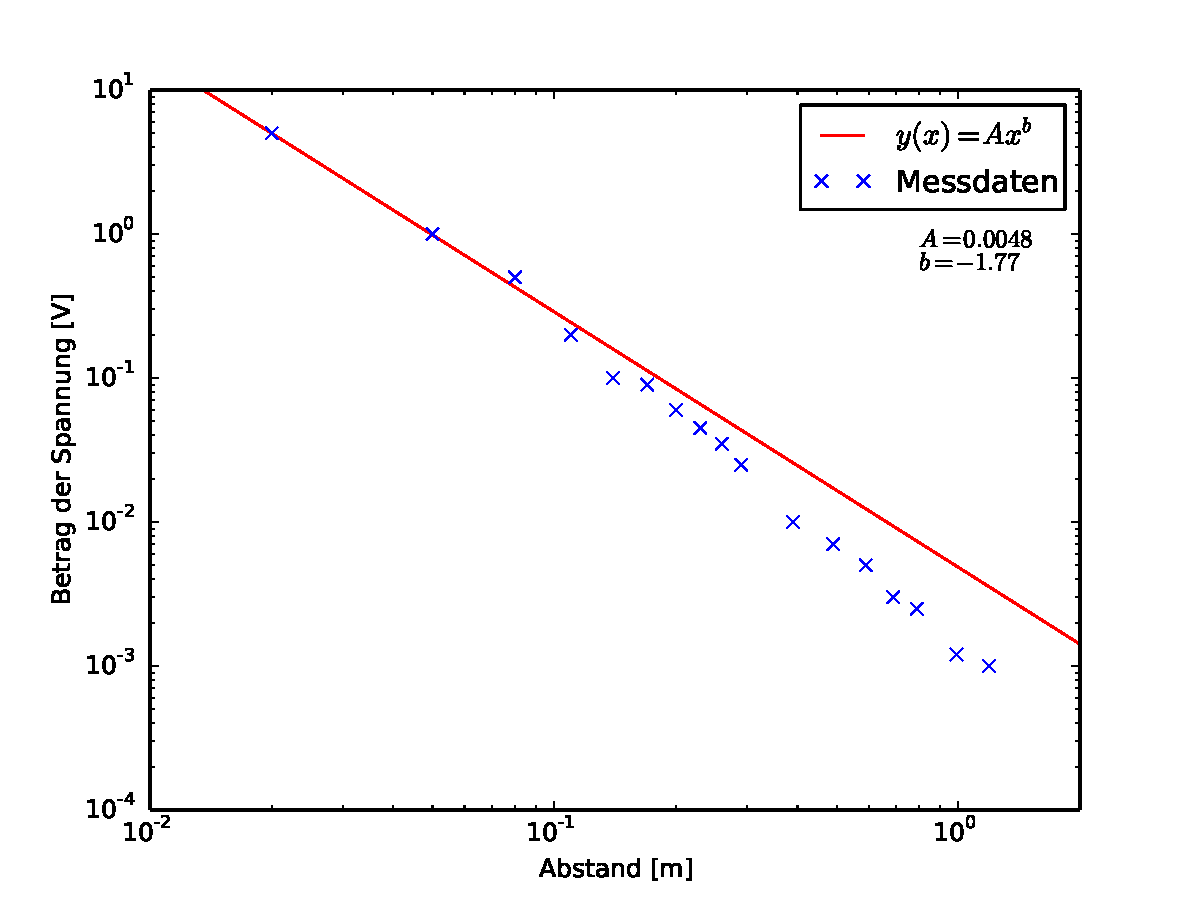
\includegraphics[width=\textwidth]{Bilder/LED_log.pdf}
		% \caption{Doppelt-logarithmische Skalierung.}
		% \label{diag:LED_log}
	% \end{subfigure}
	\caption{Ausgangsspannung des Lock-In-Verstärkers bei Messung mit der LED  bei doppelt-logarithmische Skalierung.}
	\label{diag:LED}
\end{figure}
